
\documentclass[a4paper,fleqn]{article}
\usepackage{hevea}
\usepackage[right]{eurosym}
\newif\ifpdf
\ifx\pdfoutput\undefined
  \pdffalse
  \usepackage[
    breaklinks=true,
    backref=section,
    pagebackref]{hyperref}
  \usepackage{graphicx}
  \DeclareGraphicsExtensions{.eps,.ps,.eps.gz,.ps.gz}%.png,

\else
  \pdfoutput=1
  \pdftrue
  %\usepackage[pdftex,colorlinks=true,urlcolor=blue,linkcolor=blue]{hyperref}
  \usepackage[pdftex,
    pdftitle={Design},
    pdfauthor={Christian Schuhegger},
    pdfsubject={Open Java Trading System},
    pdfkeywords={},
    pdfcreator={LaTeX with hyperref package},
    breaklinks=true,
%    backref=page,
    pagebackref,
    bookmarksopen=true,
    pdfstartview=FitH,
    pdfpagemode={UseOutlines}]{hyperref}

  \pdfcompresslevel=9
  %\usepackage{pslatex}
  \usepackage{graphicx}
  \DeclareGraphicsExtensions{.pdf}
\fi

\hypersetup{colorlinks=false,linkcolor=blue,citecolor=blue} 
\usepackage[T1]{fontenc}
\usepackage[latin1]{inputenc}
\usepackage{lmodern}
\usepackage{fancyvrb}
\usepackage[fleqn]{amsmath}
\usepackage{amssymb}
\usepackage[left=2cm,right=4cm]{geometry}
\usepackage{listings}

\pagestyle{plain}
\setlength{\mathindent}{2em}
\setlength{\marginparwidth}{3cm}
\setlength{\tabskip}{0cm}
\tolerance=3000


\newcommand{\textem}[1]{\textit{#1}} \renewcommand{\d}{{\mathrm d}}

\newcommand{\email}[1]{$<$\texttt{#1}$>$}
\newcommand{\www}  [1]{\texttt{#1}}

\newfont{\dunh}{cmdunh10} 
\newfont{\pagd}{pagd at 10pt} 
\newcommand{\filesystempath}     [1]{\texttt{#1}}
\newcommand{\maketarget}         [1]{\texttt{#1}}
\newcommand{\statementtoexecute} [1]{\begin{quote}\texttt{#1}\end{quote}}
\newcommand{\softwareproduct}    [1]{#1}%}\textrm{
\newcommand{\cppclass}           [1]{{\it #1}}

\newcommand{\MeV}{\,\mathrm{MeV}}
\newcommand{\GeV}{\,\mathrm{GeV}}
\newcommand{\eV}{\,\mathrm{eV}}
\newcommand{\V}{\,\mathrm{V}}
\newcommand{\GeVc}{\,\mathrm{GeV}/c}
\newcommand{\MHz}{\,\mathrm{MHz}}
\newcommand{\s}{\,\mathrm{s}}
\newcommand{\Ohm}{\,\Omega}
\newcommand{\kOhm}{\,\mathrm{k}\Omega}
\newcommand{\ns}{\,\mathrm{ns}}
\newcommand{\cm}{\,\mathrm{cm}}
\newcommand{\mm}{\,\mathrm{mm}}
\newcommand{\nm}{\,\mathrm{nm}}
\newcommand{\mum}{\,\mu\mathrm{m}}
\newcommand{\mus}{\,\mu\mathrm{s}}
\newcommand{\ms}{\,\mathrm{ms}}
\newcommand{\kV}{\,\mathrm{kV}}
\newcommand{\m}{\,\mathrm{m}}
\newcommand{\mrad}{\,\mathrm{mrad}}
\newcommand{\T}{\,\mathrm{T}}
\newcommand{\K}{\,\mathrm{K}}
\newcommand{\mK}{\,\mathrm{mK}}

\newcommand{\chemical}[1]{{\mathrm{#1}}}
\newcommand{\name}[1]{\textsc{#1}}
\newcommand{\ElJa}{\name{Ellis-Jaffe}}
\newcommand{\Ellis}{\name{Ellis}}
\newcommand{\Jaffe}{\name{Jaffe}}
\newcommand{\Bjorken}{\name{Bjorken}}
\newcommand{\Primakoff}{\name{Primakoff}}
\newcommand{\Compton}{\name{Compton}}
\newcommand{\Coulomb}{\name{Coulomb}}
\newcommand{\Cabibbo}{\name{Cabibbo}}
%\newcommand{\Cherenkov}{\name{Cherenkov}}
\newcommand{\Cherenkov}{\name{\v Cerenkov}}
\newcommand{\Larmor}{\name{Larmor}}
\newcommand{\Raether}{\name{Raether}}
\newcommand{\OpenJavaTradingSystem}{\name{OpenJavaTradingSystem}}
\newcommand{\Java}{\name{Java}}
\newcommand{\Scheme}{\name{Scheme}}

%BEGIN LATEX
\newcommand{\macs}[2][]{\acs#1{#2}}
\newcommand{\macl}[2][]{\acl#1{#2}}
\newcommand{\macf}[2][]{\acf#1{#2}}
\newcommand{\mac}[2][]{\ac#1{#2}}
\newcommand{\mgls}[2][]{\gls#1{#2}}
%END LATEX

\title{Open Java Trading System\\
\Large Dokumentation
}

\author{\ahref{mailto:Christian dot Schuhegger at gmx dot de}{Christian Schuhegger}}

\date{4th December 2004}

\begin{document}

\pdfbookmark[0]{OpenJavaTradingSystem}{beg}% beg.0
\maketitle

\pdfbookmark[1]{Contents}{cont}%
%XBEGIN LATEX
\tableofcontents
%XEND LATEX
%\begin{htmlonly}
%\begin{thecontent}\input{ojts-hva.toc}\end{thecontent}
%\end{htmlonly}

\lstset{commentstyle=\textit, stringstyle=\upshape,showspaces=false}
\lstset{language=java}
\section{Java Data Objects}

\noindent In the Java Data Object layer you will find classes that
serve as the representation of the data and meta-data which is
used as the basis for later analysis. Because the data is represented
in different forms, e.g. as java objects, as rows in a database or as
xml files we use the object relational mapping tool
\href{http://www.castor.org/}{castor} to map between the diferent
representations.

\subsection{Meta-Data Classes}

\noindent In the end we want to be able to do data analysis on the
market data. We gather the market data via publicly available services
like yahoo finance or onvista. These services we call observers,
because they observe the market activities. 

One given equity which is uniquely identified by its ISIN number is
traded at several different markets, e.g. the NYSE or the German
XETRA. Therefore at a given time there is not one single price for a
given equity, but there are as many prices as there are
markets. Actually these price differences will be used by arbitraters
to generate profits.

Up to now we have already the concepts ``Observer'', ``MarketPlace'' and
``Equity'' which we all need to describe. In the meta data layer there
is therefore a class for every such concept. These classes all derive
from the general base class \lstinline!Subject!:
\begin{lstlisting}[frame=trbl]{}
public class Subject {
	private int    id;
	
	private String name;
	private String description;
	private String urlSources;
}
\end{lstlisting}
The \lstinline!name! uniquely identifies the subject in its category (Observer,
MarketPlace or Equity). The \lstinline!description! is used to provide some documentation
about the subject and the \lstinline!urlSources! is a white-space
separated list of urls to web resources which are relevant for the
given subject.

The derived concepts \lstinline!Observer!, \lstinline!MarketPlace! and
\lstinline!Equity! currently all do not provide any additional
information:
\begin{lstlisting}[frame=trbl]{}
public class Observer    extends Subject {
}
public class MarketPlace extends Subject {
}
public class Equity      extends Subject {
}
\end{lstlisting}

Above we said that equities are uniquely identified by their ISIN
number. But ISIN numbers are not the only means that people use to
identify equities. In Germany for example there are WKN numbers in
widespread use or yahoo uses its own yahoo symbols to identify
securities, companies or indices. In order to be able to find equities
via these alternative identifiers we introduced the concept of aliases:
\begin{lstlisting}[frame=trbl]{}
public class Alias {
	protected int              id;
	
	protected Subject          subject;
	protected AliasType        type;
	protected MarketPlace      market;
	protected String           alias;
}
\end{lstlisting}
Normally there is an authority that assigns these alternative
identifiers. These authorities are identified via the
\lstinline!AliasType! element and we will have a look at them in a
minute. Sometimes an alias is closely related to a market place that
uses them and the \lstinline!MarketPlace! element can be used to
express this close relation. The alias itself is of type
\lstinline!String! so that it can be used to express anything.

\begin{lstlisting}[frame=trbl]{}
public class AliasType {
	protected int      id;

	protected String   name;
	protected Observer observerLink;
	protected String   description;
	protected String   urlSource;
}
\end{lstlisting}
If there is such a central authority which assigns aliases you will
have to define the authority as a element of type
\lstinline!Observer!. The \lstinline!description! and
\lstinline!urlSource! have similar meanings as in the case of the
\lstinline!Subject! class.

In general elements of type \lstinline!Subject! have more details as
there were given as properties in the \lstinline!Subject! class. These
additional properties can be described via the \lstinline!Property!
class.
\begin{lstlisting}[frame=trbl]{}
public class Property {
	protected int                 id;

	protected PropertyType        type;
	protected String              name;
	protected String              description;
}
\end{lstlisting}
All properties that express a quantity of similar meaning are of the
same \lstinline!PropertyType!. You can think of properties of the same
type as of quantities with the same unit or at least with units that
can be converted into eachother.
\begin{lstlisting}[frame=trbl]{}
public class PropertyType {
	protected int    id;

	protected String name;
	protected String description;
}
\end{lstlisting}
As an example we can take the properties ``min-day-price'',
``max-day-price'', ``opening-price'' and ``closing-price''. All of
these properties are of the same type ``price''. These quantities do not
necessarily have the same unit, e.g. sometimes they are expressed in
\euro{} and sometimes they are expressed in \$, but you can convert
from the one to the other.

While we are just talking about units. There is also a class that
describes units:
\begin{lstlisting}[frame=trbl]{}
public class Unit {
	protected int          id;

	protected String       name;
	protected PropertyType propertyTypeLink;
}
\end{lstlisting}
There is a \lstinline!propertyTypeLink! in order to express that all
units that have the same \lstinline!propertyTypeLink! can be converted
back and forth to oneanother.

In order to configure the data import methods there are classes
\lstinline!DataSource! and \lstinline!DataSourceType!. The
\lstinline!DataSourceType! can be seen more or less as a ``mime
type''. You should be able to read from all data sources with the same
\lstinline!DataSourceType! with the same data source handler code.
\begin{lstlisting}[frame=trbl]{}
public class DataSourceType {
	protected int    id;

	protected String name;
	protected String description;
}
\end{lstlisting}
The \lstinline!DataSource! class looks as follows:
\begin{lstlisting}[frame=trbl]{}
public class DataSource {
	protected int             id;

	protected DataSourceType  type;
	protected String          url;
	protected String          description;
	protected Observer        observerLink;
	protected String          handlerClassName;
}
\end{lstlisting}
The \lstinline!url! element should be seen as a pattern that the
handler code can use to retrieve actual data for a specific
equity. The \lstinline!observerLink! tells you which service provides
the data and the \lstinline!handlerClassName! will be used to create a
handler class via \Java{} reflection.

But because the handler class will need more information in order to
do its job, which it will have to retrieve from the database there is
an additional configuration class called
\lstinline!ObserverDataSourceConfiguration!. When the handler is
called it will use this configuration data to determin which data can
be found in which position on the retrieved page.
\begin{lstlisting}[frame=trbl]{}
public class ObserverDataSourceConfiguration {
	protected int         id;

	protected Property    property;
	protected MarketPlace observedAt;
	protected DataSource  observerDataSource;
	protected Unit        unit;
	protected String      colu;
}
\end{lstlisting}
The \lstinline!property! tells the handler which property is
configured via this \lstinline!ObserverDataSourceConfiguration!
instance. Because a given observer can observe several markets we need
to tell the handler which market-place we are talking about. The
handler needs to be informed which unit the property is measured in
aswell. The String field \lstinline!colu! is there to
provide additional information to handlers in a free format. The name
``colu'' reminds of its origin. Initially it was meant to point to
a column in a csv file format.


\subsection{Data Classes}

\noindent All data classes derive from one common base class:
\begin{lstlisting}[frame=trbl]{}
public class DataItem {
	protected int                             id;

	protected Date                            time;
	protected Subject                         subject;
	protected ObserverDataSourceConfiguration source;
}
\end{lstlisting}
The data is actually what we are interested in for our later
analysis. The data that we collect is a function of time, it belongs
to a specific subject, it describes a certain aspect/property of that
subject, it is observed by an observer at a certain market-place and
finally it has a unit. All the information which is not directly
present in this class can be retrieved by following the object graph
in the \lstinline!source! element.

There are subclasses of this \lstinline!DataItem! class for the
concrete data types: Boolean, Double, Int, String and Time.


\section{Interactive usage}
\subsection{SISC a Scheme implementation in Java}

\noindent This section is here to give you a preliminary feeling of
what the project can do for you and where the project is going in the
future. The project is a pure \Java{} project and designed in such a
way that you can easily integrate its functionality into your own
applications. For my personal use I prefer to work with the
\OpenJavaTradingSystem{} functionality in an interactive
way. Therefore I've written some adapter code to be able to call the
\OpenJavaTradingSystem{} functionality from
\href{http://sisc.sourceforge.net/}{SISC}, a pure \Java{}
implementation of the algorithmic programming language
\Scheme{}\footnote{A good first introduction can be found at
  \href{http://www.ccs.neu.edu/home/dorai/t-y-scheme/t-y-scheme.html}{Teach Yourself Scheme in Fixnum Days}}. 
Other types of integration, e.g. into
\href{http://www.jython.org/}{Jython} or
\href{http://www.beanshell.org/}{BeanShell} seem to be other options.


The following explanations assume that you are in the
\OpenJavaTradingSystem{} project directory.

The first step before you can start to work with the
\OpenJavaTradingSystem{} is to start the database server in the
backgroud:
\begin{verbatim}
> java -cp lib/hsqldb.jar org.hsqldb.Server -database.0 data/jts -dbname.0 jts
\end{verbatim}
Basically this step is optional if you change the ``jdbc\_location''
property in the \filesystempath{conf/jts.properties} configuration
file to use the ``:file:'' access method. The advantage of using the
database server is that you can connect to it from several clients,
whereas if you choose to use the ``:file:'' access method only the
\OpenJavaTradingSystem{} application is able to access it.

In the project root directory you will find a modified startup
script\footnote{At the moment there is no equivalent windows script
available, but I would be happy to integrate one if you can provide me
one.} to start SISC. There is an ant task \maketarget{sisc-repl} aswell, which
you can use to start the read-eval-print loop. Now you can work
interactively with the system. Let's start with the initialization
procedure. One day this initialization procedure will be integrated
into the bash startup script, but until then you have to initialize
the system as follows:
\lstset{language=Lisp}
\begin{verbatim}
> (current-directory (getenv "sisc.home"))
> (load "sisc/functionality.scm")
> (ojts:init)
\end{verbatim}
If you start the system for the first time you also have to initialize
the content of some database tables from an xml file:
\begin{verbatim}
> (ojts:read-xml-configuration "testread.xml")
\end{verbatim}
From here on you can start retrieving data from the internet or
displaying data in a graph. All of the following commands are
independent and can be executed\footnote{For those who do not know
\Scheme{} one remark: The indentation and newlines are optional. You
can execute every command on a single line.} one by one without the
others:
\begin{verbatim}
> (ojts:fetch-data "yahoo-csv" "2004-06-01" "2004-08-23" 
                   "DE0007500001" "XETRA")
> (ojts:fetch-data "yahoo-csv" "2004-06-01" '() 
                   "DE0007500001" "XETRA")

> (ojts:get-ohlc-for-equity "yahoo-csv" "2004-06-01" "2004-07-01" 
                            "DE0007500001" "XETRA")
> (ojts:get-data-for-equity "yahoo-csv" "2004-06-01" "2004-07-01" 
                            "DE0007500001" "XETRA" *CLOSING-DAY-PRICE*)
> (ojts:get-data-for-equity "yahoo-csv" "2004-06-01" "2004-07-01" 
                            "DE0007500001" "XETRA" *TRADING-DAY-VOLUME*)
  
> (ojts:display-chart 
   (ojts:create-candlestick-chart-for-equity 
     "yahoo-csv" "2004-06-01" "2004-07-01" "DE0007500001" "XETRA"))
\end{verbatim}
All operations that require data will try to find that data in the
database. If the data cannot be found the system will try to get
the data from the web. This action is the same as what happens when
you execute the \statementtoexecute{ojts:fetch-data} statement. Here you can
see the result for one of the
\statementtoexecute{ojts:get-data-for-equity} operations from above:
\begin{verbatim}
> (ojts:get-data-for-equity "yahoo-csv" "2004-06-01" "2004-07-01" 
                            "DE0007500001" "XETRA" *TRADING-DAY-VOLUME*)
INFO - Was fetching data for 0 days therefore no commits are necessary.
(("2004-06-01" "integer" 1267190.0)
 ("2004-06-02" "integer" 2241070.0)
 ("2004-06-03" "integer" 1953370.0)
 ("2004-06-04" "integer" 2015380.0)
 ("2004-06-07" "integer" 1953470.0)
 ("2004-06-08" "integer" 1487590.0)
 ("2004-06-09" "integer" 3193410.0)
 ("2004-06-10" "integer" 1641250.0)
 ("2004-06-11" "integer" 1635660.0)
 ("2004-06-14" "integer" 2541210.0)
 ("2004-06-15" "integer" 2598440.0)
 ("2004-06-16" "integer" 1913340.0)
 ("2004-06-17" "integer" 2303420.0)
 ("2004-06-18" "integer" 3802480.0)
 ("2004-06-21" "integer" 2514830.0)
 ("2004-06-22" "integer" 1499570.0)
 ("2004-06-23" "integer" 2305450.0)
 ("2004-06-24" "integer" 4740060.0)
 ("2004-06-25" "integer" 2459800.0)
 ("2004-06-28" "integer" 2783660.0)
 ("2004-06-29" "integer" 2555130.0)
 ("2004-06-30" "integer" 4322920.0)
 ("2004-07-01" "integer" 4587870.0))
\end{verbatim}
And in figure~\ref{sample-candlestick} you can see the output
of the following chart creating command:
\begin{verbatim}
> (ojts:display-chart 
   (ojts:create-candlestick-chart-for-equity 
     "yahoo-csv" "2004-06-01" "2004-07-01" "DE0007500001" "XETRA"))
\end{verbatim}
\begin{figure}[htbp]
\caption{Sample Candlestick Chart}
\label{sample-candlestick}
\href{graphics/ojts-candlestick-chart.png}{\centerline{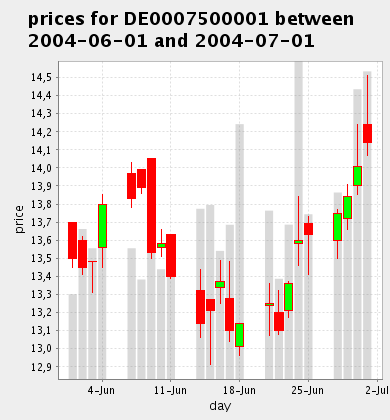
\includegraphics[width=5cm,clip=true]{graphics/ojts-candlestick-chart}}}
\end{figure}


\subsection{Using the ilisp Emacs mode}

\noindent Normally you won't work with the \Scheme{} interpreter on
the commandline. Usually one uses a more convenient environment like
the \href{http://sourceforge.net/projects/ilisp/}{ilisp} emacs
mode. If you are on a unix system probably you can get a package for
your package system to install ilisp. If you are on windows you can
follow the installation procedure described at
\href{http://cl-cookbook.sourceforge.net/windows.html}{Setting up an
IDE with Emacs on Windows}.

As soon as you have a working ilisp mode you have to add the following
section to your .emacs file in order to make ilisp work together with
SISC:
\begin{verbatim}
(setq ilisp-*use-fsf-compliant-keybindings* nil)

(add-hook 'ilisp-load-hook
          '(lambda ()
	     (defdialect sisc "SISC Scheme"
	       scheme
	       (setq ilisp-program "~/workspace/OpenJavaTradingSystem/sisc-ilisp.sh")	; assume scheme is in path.
	       (setq comint-prompt-regexp "^> ")
	       (setq ilisp-eval-command
		     "(car (list (eval (read (open-input-string \"%s\"))) \"%s\" \"%s\"))"
		     ilisp-package-command "%s"
		     ilisp-macroexpand-command "(expand '%s);%s"
		     ilisp-trace-command "(trace %s);%s"
		     ilisp-untrace-command "(untrace %s);%s"
		     ilisp-directory-command  "(current-directory);%s"
		     ilisp-set-directory-command "(current-directory \"%s\")"
		     ilisp-describe-command "(describe %s)"
		     comint-ptyp t
		     comint-always-scroll t
		     ilisp-last-command "*"
		     ))))
	       

(set-default 'auto-mode-alist
             (append '(("\\.scm$"  . scheme-mode)
		       ("\\.sisc$" . scheme-mode))
                     auto-mode-alist))

(setq scheme-mode-hook '(lambda () (require 'ilisp)))
\end{verbatim}
You have to adapt the ilisp-program line to suite your set-up. 

Now you are ready to use the \Scheme{} interface to the
\OpenJavaTradingSystem{} from within the ilisp emacs mode. In emacs
use \statementtoexecute{M-x run-ilisp} and when you're asked for the
``Dialect'' answer with ``sisc''. This should startup the \Scheme{}
interpreter in your emacs window.

Details about the usage of the ilisp emacs mode can be found in its
\href{http://www.xemacs.org/Documentation/packages/html/ilisp.html}{manual}.

And finally in figure~\ref{emacs-ilisp-sisc} is a screenshot of using
the \OpenJavaTradingSystem{} via the \Scheme{} interface from within emacs.
\begin{figure}[htbp]
\caption{Emacs -- Ilisp -- SISC}
\label{emacs-ilisp-sisc}
\href{graphics/emacs-ilisp-sisc.png}{\centerline{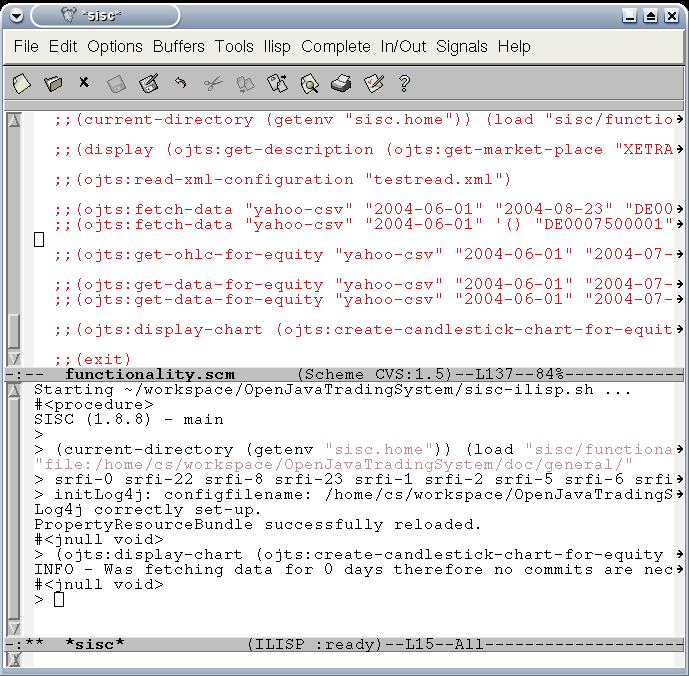
\includegraphics[width=9cm,clip=true]{graphics/emacs-ilisp-sisc}}}
\end{figure}

\subsection{Configuring the SQLExplorer plugin for Eclipse}

\noindent As mentioned above, the advantage of starting the database
server instead of using the ``:file:'' access method is that you can
connect to the database via the network with other programs aswell. I
personally have started to use the
\href{https://sqlexplorer.dev.java.net/}{SQLExplorer} plugin for the
Eclipse IDE. The packed distribution can be found on their website
under ``Documents \& files''. In order to install it you only have to
unpack the distribution into the Eclipse directory. 

After a restart of Eclipse you will have to open the SQLExplorer
perspective. At the left top in the ``Drivers'' tab you have to
configure the ``HSQLDB Server'' by clicking on it with the right mouse
button and selecting ``Change the selected Driver''. Look at the
screen shot in figure~\ref{sqlexplorer-hsqldb-driver} to see how you should
configure these fields. 
\begin{figure}[htbp]
\caption{SQLExplorer HSQLDB driver configuration}
\label{sqlexplorer-hsqldb-driver}
\href{graphics/sqlexplorer-hsqldb-driver.png}{\centerline{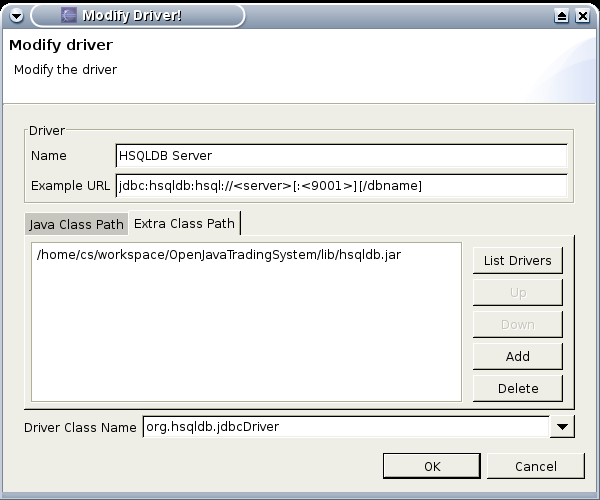
\includegraphics[width=5cm,clip=true]{graphics/sqlexplorer-hsqldb-driver}}}
\end{figure}
After adding the right jar file you have to click the ``List Drivers''
button and select the hsqldb JDBC driver as you can see in the screen
shot.

The next step is to configure in the ``Aliases'' tab an alias for your
database. In screen shot~\ref{sqlexplorer-hsqldb-alias} you can see
what to put there.
\begin{figure}[htbp]
\caption{SQLExplorer HSQLDB alias configuration}
\label{sqlexplorer-hsqldb-alias}
\href{graphics/sqlexplorer-hsqldb-alias.png}{\centerline{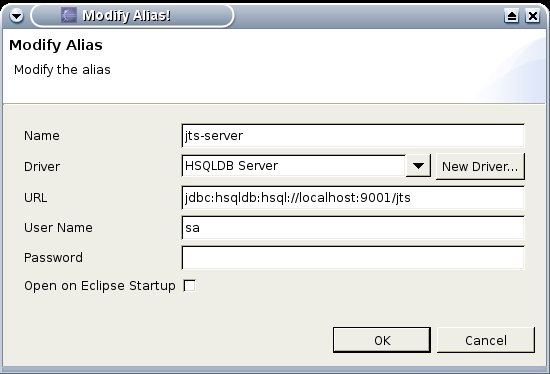
\includegraphics[width=5cm,clip=true]{graphics/sqlexplorer-hsqldb-alias}}}
\end{figure}

Now you are ready to connect to the database (make sure the server is
running) via the ``Connections'' tab at the left bottom. As soon as
you are connected you will see the ``Database Structure View''
tab. Use this view to browse through the available tables in the
database. 

As next step you can click with your right mouse button on a table
name and use ``Generate Select in SQL Editor'' to open a prefilled SQL
Editor tab. From here on you should be able to find yourself your way
through the functionality of this plugin.

\end{document}
